\documentclass[10pt, aspectratio=169]{beamer}

% THEME -------------------------------------------------------
\usetheme{metropolis}       % Modern, clean
\usecolortheme{default}

% PACKAGES ----------------------------------------------------
\usepackage{amsmath, amssymb, amsthm}
\usepackage{multicol}
\usepackage{multirow}
\usepackage{array}
\usepackage{graphicx}
\usepackage{booktabs}
\usepackage{algorithm}
\usepackage[noend]{algpseudocode}
\usepackage{tikz,pgfplots}
\usetikzlibrary{positioning,backgrounds,calc,trees}
\pgfdeclarelayer{map}
\pgfdeclarelayer{square}
\pgfsetlayers{map,square,main}
\usepackage{hyperref}
\usepackage[T1]{fontenc}
\usepackage{libertinus}
\usepackage[normalem]{ulem}
\usepackage[most]{tcolorbox}
\tcbuselibrary{skins}

% \usepackage{apalike}
\bibliographystyle{apalike}

% \usepackage[
%     backend=biber,
%     style=authoryear,   % or numeric, ieee, etc.
%     maxnames=10
% ]{bibtex}
% \addbibresource{refs.bib}


\newcommand{\cB}{\mathcal{B}}
\newcommand{\cI}{\mathcal{I}}

\newcommand{\pref}{\mathrm{pref}}
\newcommand{\zeroone}{\ensuremath{\{0, 1\}}}

\definecolor{darkgreen}{RGB}{0,130,0}

% remove the background bar completely
\setbeamertemplate{frametitle}{%
  \nointerlineskip%
  \vspace{0.8em}%
  % \hspace{-0.1em}%
  {\usebeamerfont{frametitle}\color{navyblue}\insertframetitle}%
}

% define the color you want (navy blue)
\definecolor{navyblue}{RGB}{0,45,95}
\setbeamerfont{frametitle}{size=\LARGE,series=\bfseries}

% DOCUMENT ----------------------------------------------------
\begin{document}

\begin{frame}[plain]
\setbeamercolor{background canvas}{bg=white}

\begin{tikzpicture}[remember picture,overlay]

% ---- MAIN TITLE ----
\node[anchor=center] at ([yshift=15mm]current page.center) {
    \begin{minipage}{\linewidth}
        \centering
        {\LARGE\bfseries New Framework for Structure-Aware PSI \\[2mm]
        from Distributed Function Secret Sharing}
    \end{minipage}
};

% ---- AUTHORS (shift downward from center) ----
\node[anchor=center] at ([yshift=-10mm]current page.center) {
    \begin{minipage}{0.9\linewidth}
        \centering
        {\large
            Dung Bui\textsuperscript{1} \quad
            Gayathri Garimella\textsuperscript{2} \quad
            Peihan Miao\textsuperscript{2} \quad
            Phuoc Pham\textsuperscript{2}
        }\\[3mm]
        {\small
            \textsuperscript{1} Sorbonne Universit\'e \\[-1mm]
            \textsuperscript{2} Brown University
        }
    \end{minipage}
};

% ---- CONFERENCE NAME (shift further down) ----
\node[anchor=center] at ([yshift=-25mm]current page.center) {
    {\large Asiacrypt 2025}
};

\end{tikzpicture}
\end{frame}

\begin{frame}<1-2>
\frametitle{Private Set Intersection}

Private Set Intersection \cite{meadows1986more,freedman2004efficient} outputs {\color{blue} set intersection} while hiding the {\color{red} remaining elements}.
\vspace{15em} % text push-down

\begin{tikzpicture}[remember picture,overlay]
% --- Alice image ---
\node[anchor=north west, xshift=1.5cm, yshift=-2.5cm]
    (aliceimg)
    at (current page.north west)
    {\includegraphics[width=0.13\linewidth]{../Resources/Alice.png}};

% --- Bob image ---
\node[anchor=north east, xshift=-1.5cm, yshift=-2.5cm]
    (bobimg)
    at (current page.north east)
    {\includegraphics[width=0.15\linewidth]{../Resources/Bob.png}};

% --- Table styling for PSI lists ---
\tcbset{
    mytablebox/.style={
        enhanced,
        colback=white,
        colframe=black!60,
        boxrule=0.7pt,
        arc=3mm,
        left=3mm,right=3mm,top=2mm,bottom=2mm,
        width=2cm,
        halign=center,
    }
}


% --- Alice table ---
\node[anchor=north west, xshift=1.5cm, yshift=-4.5cm] at (current page.north west) {
    \begin{tcolorbox}[mytablebox]
        \only<1>{Emma}\only<2>{\textcolor{gray!60}{Emma}} \\
        {\color{darkgreen} Daniel} \\
        \only<1>{Olivia}\only<2>{\textcolor{gray!60}{Olivia}} \\
        \only<1>{Michael}\only<2>{\textcolor{gray!60}{Michael}} \\
        {\color{darkgreen} Sophia}
    \end{tcolorbox}
};

% % --- Bob table ---
\node[anchor=north east, xshift=-1.5cm, yshift=-4.5cm] at (current page.north east) {
    \begin{tcolorbox}[mytablebox]
        {\color{darkgreen} Daniel} \\
        \only<1>{James}\only<2>{\textcolor{gray!60}{James}} \\
        {\color{darkgreen} Sophia} \\
        \only<1>{William}\only<2>{\textcolor{gray!60}{William}} \\
        \only<1>{Ava}\only<2>{\textcolor{gray!60}{Ava}}
    \end{tcolorbox}
};

\node[anchor=center, yshift=-1cm] (intersectbox) at (current page.center) {
    \begin{tcolorbox}[mytablebox]
        Daniel \\
        Sophia
    \end{tcolorbox}
};

\visible<2>{
  % Curved arrow from intersection table to Alice
  \draw[->, ultra thick, navyblue]
    ([xshift=-0.2cm,yshift=0.1cm]intersectbox.west)
      to[out=200,in=-30] ([xshift=0.2cm,yshift=-0.6cm]aliceimg.east);
}

\end{tikzpicture}

\end{frame}

\begin{frame}
\frametitle{Many Applications}

\begin{columns}[T]
  \begin{column}{0.42\textwidth}
  { \Large
  \begin{itemize}
      \item Password Monitoring
      \vspace{0.5cm}
      \item Contact Discovery
      \vspace{0.5cm}
      \item Biometric Search
      \vspace{0.5cm}
      \item Inventory Matching
      \vspace{0.5cm}
      \item $\ldots$
  \end{itemize}
  }
  \end{column}
  \begin{column}{0.58\textwidth}
    \centering
    \begin{tikzpicture}
      \node[anchor=center] (imgbase) at (0,5) {};
      \node[anchor=center, rotate=2] at ([xshift=0.8cm,yshift=0.7cm]imgbase)
        {\includegraphics[width=0.85\linewidth]{password-monitoring.png}};
      \node[anchor=center, rotate=-3] at ([xshift=1cm,yshift=-0.3cm]imgbase)
        {\includegraphics[width=0.73\linewidth]{inventory-matching.png}};
      \node[anchor=center] at ([yshift=-2cm]imgbase)
        {\includegraphics[width=0.98\linewidth]{contact-discovery.png}};
    \end{tikzpicture}
  \end{column}
\end{columns}
\end{frame}

\begin{frame}
\frametitle{Privacy-Preserving Ride Sharing}
\only<1,2>{
  Sometimes output requires {\color{darkgreen} close enough} elements, instead of {\color{red} exactly matched}.
}
\only<3>{
  Putting {\color{red} every points} and running plain PSI is too costly!
}
\vspace{15em}
\begin{tikzpicture}[overlay, remember picture]

%% Maps (background layer)
\begin{pgfonlayer}{map}
\node[anchor=north west, xshift=1.5cm, yshift=-4cm] at (current page.north west) {
  \includegraphics[width=5cm]{../Resources/melbourne_street_map.jpg}
};
\node[anchor=north east, xshift=-1.5cm, yshift=-4cm] at (current page.north east) {
  \includegraphics[width=5cm]{../Resources/melbourne_street_map.jpg}
};
\end{pgfonlayer}

\visible<1,2>{
%% Cars (main layer)
\node (car1) [anchor=north west, xshift=1.8cm, yshift=-5cm] at (current page.north west) {
  \includegraphics[width=0.8cm]{../Resources/Car_red.PNG}
};
\node (car2) [anchor=north west, xshift=3cm, yshift=-6.6cm] at (current page.north west) {
  \includegraphics[width=0.8cm]{../Resources/Car_red.PNG}
};
\node (car3) [anchor=north west, xshift=5.4cm, yshift=-5.8cm] at (current page.north west) {
  \includegraphics[width=0.8cm]{../Resources/Car_red.PNG}
};
\node (car4) [anchor=north west, xshift=3.6cm, yshift=-5.4cm] at (current page.north west) {
  \includegraphics[width=0.8cm]{../Resources/Car_red.PNG}
};
}

%% Light-green squares + δ arrows (middle layer)
\only<2>{
\begin{pgfonlayer}{square}
  % car1
  \node[fill=green!10,minimum size=1cm,inner sep=0pt] (sq1) at (car1) {};
  % \draw[<->] ([xshift=0.03cm, yshift=0.15cm]sq1.south west) -- ([xshift=-0.03cm, yshift=0.15cm]sq1.south east)
  %   node[midway, fill=green!20, inner sep=1pt] {{\scriptsize $\delta$}};

  % car2
  \node[fill=green!10,minimum size=1cm,inner sep=0pt] (sq2) at (car2) {};
  % \draw[<->] ([xshift=0.03cm, yshift=0.15cm]sq2.south west) -- ([xshift=-0.03cm, yshift=0.15cm]sq2.south east)
  %   node[midway, fill=green!20, inner sep=1pt] {{\scriptsize $\delta$}};

  % car3
  \node[fill=green!10,minimum size=1cm,inner sep=0pt] (sq3) at (car3) {};
  % \draw[<->] ([xshift=0.03cm, yshift=0.15cm]sq3.south west) -- ([xshift=-0.03cm, yshift=0.15cm]sq3.south east)
  %   node[midway, fill=green!20, inner sep=1pt] {{\scriptsize $\delta$}};

  % car4
  \node[fill=green!10,minimum size=1cm,inner sep=0pt] (sq4) at (car4) {};
  % \draw[<->] ([xshift=0.03cm, yshift=0.15cm]sq4.south west) -- ([xshift=-0.03cm, yshift=0.15cm]sq4.south east)
  %   node[midway, fill=green!20, inner sep=1pt] {{\scriptsize $\delta$}};
\end{pgfonlayer}
}
\only<3>{
\begin{pgfonlayer}{square}
  % Fill each square with a 4x4 grid of cars
  \foreach \dy/\shift in {-0.48/0, -0.24/0.12, 0/0, 0.24/0.12, 0.48/0} {
    \foreach \dx in {-0.36,-0.12,0.12,0.36} {
      \node at ([xshift=\dx cm,yshift=\dy cm]car1) {\includegraphics[width=0.2cm]{../Resources/Car_red.PNG}};
      \node at ([xshift=\dx cm,yshift=\dy cm]car2) {\includegraphics[width=0.2cm]{../Resources/Car_red.PNG}};
      \node at ([xshift=\dx cm,yshift=\dy cm]car3) {\includegraphics[width=0.2cm]{../Resources/Car_red.PNG}};
      \node at ([xshift=\dx cm,yshift=\dy cm]car4) {\includegraphics[width=0.2cm]{../Resources/Car_red.PNG}};
    }
  }
  % keep a light boundary for the squares
  \node[draw=green!50,minimum size=1cm,inner sep=0pt] at (car1) {};
  \node[draw=green!50,minimum size=1cm,inner sep=0pt] at (car2) {};
  \node[draw=green!50,minimum size=1cm,inner sep=0pt] at (car3) {};
  \node[draw=green!50,minimum size=1cm,inner sep=0pt] at (car4) {};
\end{pgfonlayer}
}

%% Passengers (main layer)
\node[anchor=north east, xshift=-1.8cm, yshift=-4.6cm] at (current page.north east) {
  \includegraphics[width=1cm]{../Resources/Smile_emoji.PNG}
};
\node[anchor=north east, xshift=-2.5cm, yshift=-5.7cm] at (current page.north east) {
  \includegraphics[width=1cm]{../Resources/Smile_emoji.PNG}
};
\node[anchor=north east, xshift=-3.4cm, yshift=-6.4cm] at (current page.north east) {
  \includegraphics[width=1cm]{../Resources/Smile_emoji.PNG}
};
\node[anchor=north east, xshift=-4.0cm, yshift=-5cm] at (current page.north east) {
  \includegraphics[width=1cm]{../Resources/Smile_emoji.PNG}
};
\node[anchor=north east, xshift=-5.3cm, yshift=-4.2cm] at (current page.north east) {
  \includegraphics[width=1cm]{../Resources/Smile_emoji.PNG}
};

\end{tikzpicture}
\end{frame}

\begin{frame}
\frametitle{Structure-Aware Private Set Intersection} 
\only<1>{
Structure-Aware Private Set Intersection \cite{garimella2022structure} outputs intersection between:
\begin{itemize}
  \item Sender's set of {\color{teal} points}
  \item Receiver's set of {\color{orange} structures} e.g. balls, intervals
\end{itemize}
}
\only<2,3>{
In this work, we focus on {\color{orange} $L_\infty$} distance metric, with ball diameter {\color{orange}$\delta$}. \\
For example, in a 2D plane, the structures are {\color{teal} squares} of edge size $\delta$.
}
\vspace{15em}

\begin{tikzpicture}[overlay, remember picture]
  % --- Alice image ---
  \node[anchor=north west, xshift=1.8cm, yshift=-2.9cm]
      (aliceimg)
      at (current page.north west)
      {\includegraphics[width=0.13\linewidth]{../Resources/Alice.png}};

  % --- Bob image ---
  \node[anchor=north east, xshift=-1.8cm, yshift=-2.9cm]
      (bobimg)
      at (current page.north east)
      {\includegraphics[width=0.15\linewidth]{../Resources/Bob.png}};

  % === Alice's plane (structures) ===
  % A rectangle under Alice
    \node[anchor=north, draw, very thin,
          minimum width=4cm, minimum height=2.5cm]
        (aliceplane)
        at ([yshift=-0.8cm]aliceimg.south)
        {};

    % Light-green squares on Alice's plane (random placement, uniform size)
    \foreach \x/\y in {
      0.7/0.6,
      1.5/1.8,
      3.1/1.5,
      2.4/0.4,
      2.9/2.2
    }{
      \node[fill=green!30, minimum size=0.5cm, inner sep=0pt]
        at ($(aliceplane.south west) + (\x cm,\y cm)$) {};
    }

    % === Bob's plane (points) ===
    % A rectangle under Bob
    \node[anchor=north, draw, very thin,
          minimum width=4cm, minimum height=2.5cm]
        (bobplane)
        at ([yshift=-0.8cm]bobimg.south)
        {};

    % 5 visible yellow points on Bob's plane
  \foreach \x/\y in {0.8/0.7, 2.0/0.9, 3.0/1.5, 1.3/1.9, 2.6/2.1} {
      \fill[yellow!80!orange]
        ($(bobplane.south west) + (\x cm,\y cm)$) circle (0.07cm);
      \draw
        ($(bobplane.south west) + (\x cm,\y cm)$) circle (0.07cm);
    }

    \visible<3>{
    % === Merged plane (points inside at least one square) ===
    \node[anchor=north, draw, very thin,
          minimum width=4cm, minimum height=2.5cm]
        (mergeplane)
        at ($ (aliceimg.south)!0.5!(bobimg.south) + (0,1cm)$)
        {};

    % Squares that actually contain points (empty ones removed)
      \foreach \x/\y in {
        0.7/0.6,
        1.5/1.8,
        3.1/1.5
      }{
        \node[fill=green!30, minimum size=0.5cm, inner sep=0pt]
          at ($(mergeplane.south west) + (\x cm,\y cm)$) {};
      }

    % Points kept after intersecting with squares
      \foreach \x/\y in {0.8/0.7, 1.3/1.9, 3.0/1.5} {
        \fill[yellow!80!orange]
          ($(mergeplane.south west) + (\x cm,\y cm)$) circle (0.07cm);
        \draw
          ($(mergeplane.south west) + (\x cm,\y cm)$) circle (0.07cm);
      }

      % Arrow showing merged result sent to Alice
      \draw[->,thick,green!60!black]
        ([xshift=-0.05cm]mergeplane.west) to[out=180,in=0] ([xshift=0.2cm]aliceimg.east);
      }

    \end{tikzpicture}

\end{frame}

\begin{frame}
\frametitle{Illustration in this talk}
We consider 1-dimension, 1-sided interval, in a domain of bit length $u$.
Alice is the receiver.
\vspace{1em}

\hspace{6em}\begin{tikzpicture}[scale=1.0]

%% --- Top cartoon face (replace with your image) ---
\node at (0,1.8) {\includegraphics[width=1.2cm]{../Resources/Bob.png}};

%% --- Bottom cartoon face ---
\node at (0,-1.8) {\includegraphics[width=1.2cm]{../Resources/Alice.png}};

%% --- Axis line ---
\draw[-, thick] (0,0) -- (8,0);

%% --- Red interval (Alice interval) ---
\draw[line width=5pt, red!60, rounded corners=3pt] (0,-0.1) -- (5,-0.1);

%% --- Green marked points ---
\foreach \x in {1, 2.3, 3.8, 6, 7} {
    \fill[green!70!black] (\x,0) circle (3pt);
}

%% --- Green arrows above each point ---
\foreach \x in {1, 2.3, 3.8, 6, 7} {
    \draw[very thick, green!70!black, ->] (\x,1.1) -- (\x,0.25);
}

%% --- Green arrows above each point ---
\draw[very thick, green!70!black, ->] (5,-1.1) -- (5,-0.4);
\node at (5,-1.3) {$\alpha$};
\node at (-0.2, -0.2) {$0$};
\node at (8.2, -0.2) {$2^u-1$};
\end{tikzpicture}
\end{frame}


\begin{frame}
\frametitle{Related Works: FSS-based Approach} 
\textbf{Structure-Aware Private Set Intersection:} Current line of work uses Function Secret Sharing.
\begin{itemize}
    \item Introduced in \cite{garimella2022structure}, with application to fuzzy mapping.
    \item Extended to malicious security in \cite{garimella2023malicious}.
    \item Computationally efficient: \cite{garimella2024computation}.
    \item \textbf{This work}: Concrete efficiency and implementation!
\end{itemize}
\textbf{Fuzzy Private Set Intersection}: Techniques based on:
\begin{itemize}
    \item GC or FHE: \cite{richardson2024fuzzy, son2025doubly, uzun2021fuzzy}.
    \item Additive Homomorphic Encryption: \cite{van2024fuzzy, gao2024efficient}.
    \item Symmetric Key Techniques: \cite{zhang2025fast}, \cite{van2025fuzzy}.
\end{itemize}
\end{frame}

\newcolumntype{L}{>{\hspace{1em}}l}
\newcommand{\winning}[1]{{\color{darkgreen} #1\times}}


\begin{frame}
\frametitle{Our Contribution} 

\begin{itemize}
    \item Remove $\kappa$ overhead in Structure-aware PSI for $L_\infty$ metric distance.
    \item New trade-off in tree search, better control for WAN settings.
    \item Implementation in Rust.
\end{itemize}


\begin{table}[]
    \centering
    \resizebox{0.8\textwidth}{!}{
    \begin{tabular}{|c|c|c|L|L|L|L|L|L|}
        \hline
               \multirow{2}{*}{Set size} & \multirow{2}{*}{Radius} & \multirow{2}{*}{Protocol} & \multicolumn{2}{c|}{$d = 2$} & \multicolumn{2}{c|}{$d = 3$} & \multicolumn{2}{c|}{$d = 4$} \\
         % \cline{4-9}
         & & & \multicolumn{1}{c|}{Comm (MB)} & \multicolumn{1}{c|}{Time (s)} & \multicolumn{1}{c|}{Comm (MB)} & \multicolumn{1}{c|}{Time (s)} & \multicolumn{1}{c|}{Comm (MB)} & \multicolumn{1}{c|}{Time (s)}\\
          \hline
         \multirow{15}{*}{$2^{16}$} & \multirow{3}{*}{$10$} & \cite{van2024fuzzy} & \textbf{264} & 226 & \textbf{396} & 385 & \textbf{528} & \textbf{640} \\ 
         & & \cite{gao2024efficient} & 1,924 & 673 & 2,859 & 1,004 & 3,796 & 1,328 \\ 
         & & Ours & 436 & $\textbf{43.7}^{\winning{5.17}}$ & 1,165 & $\textbf{146}^{\winning{2.63}}$ & 4,737 & 992 \\ 
         \cline{2-9}
         & \multirow{3}{*}{$30$} & \cite{van2024fuzzy} & 768 & 593 & \textbf{1,151} & 1,004 & \textbf{1,535} & \textbf{1,562} \\ 
         & & \cite{gao2024efficient} & 5,488 & 1,645 & 8,205 & 2,390 & 10,924 & 3,254 \\ 
         & & Ours & $\textbf{568}^{\winning{1.35}}$ & $\textbf{61.1}^{\winning{9.71}}$ & 2,162 & $\textbf{236}^{\winning{4.26}}$ & 13,633 & 1,992 \\ 
         \cline{2-9}
         & \multirow{3}{*}{$60$} & \cite{van2024fuzzy} & 1,523 & 1,152 & 2,284 & 1,892 & \textbf{3,045} & \textbf{2,974} \\ 
         & & \cite{gao2024efficient} & 10,834 & 3,222 & 16,224 & 4,482 & 21,616 & 6,042 \\ 
         & & Ours & $\textbf{612}^{\winning{2.48}}$ & $\textbf{76.0}^{\winning{15.2}}$ & $\textbf{2,229}^{\winning{1.02}}$ & $\textbf{294}^{\winning{6.44}}$ & 13,721 & 3,201 \\ 
         \cline{2-9}
         & \multirow{3}{*}{$120$} & \cite{van2024fuzzy} & 3,302 & 2,286 & 4,549 & 3,684 & \textbf{6,065} & 5,788 \\ 
         & & \cite{gao2024efficient} & 21,526 & 6,027 & 32,262 & 8,868 & -- & -- \\ 
         & & Ours & $\textbf{770}^{\winning{4.29}}$ & $\textbf{111}^{\winning{20.6}}$ & $\textbf{3,830}^{\winning{1.18}}$ & $\textbf{460}^{\winning{8.01}}$ & 32,381 & $\textbf{4,770}^{\winning{1.21}}$ \\ 
         \cline{2-9}
         & \multirow{3}{*}{$250$} & \cite{van2024fuzzy} & 6,304 & 4,804 & 9,456 & 8,006 & \textbf{12,608} & 12,191 \\ 
         & & \cite{gao2024efficient} & -- & -- & -- & -- & -- & -- \\ 
         & & Ours & $\textbf{814}^{\winning{7.74}}$ & $\textbf{178}^{\winning{27.0}}$ & $\textbf{3,896}^{\winning{2.42}}$ & $\textbf{607}^{\winning{13.2}}$ & 32,470 & $\textbf{7,089}^{\winning{1.72}}$ \\ 
         \hline
    \end{tabular}}
    \caption{\small Experimental results for fuzzy PSI with $\ell_{\infty}$ distance. Our speedup factor, compared to~\cite{van2024fuzzy,gao2024efficient}, is highlighted in \textcolor{darkgreen}{green}.
    The entries filled with dash -- means the programs run out of memory.}
%    cannot be run due to RAM limit.\dung{maybe darkgreen is good color?}} \phuoc{I agree}
    \label{tab:experimental-results}
\end{table}

\end{frame}

\begin{frame}
\frametitle{Road map}
We consider 1-dimension, 1-sided interval.

\vspace{1em}

\begin{tikzpicture}[scale=1.0]

%% --- Top cartoon face (replace with your image) ---
\node at (0,1.8) {\includegraphics[width=1.2cm]{../Resources/Bob.png}};

%% --- Bottom cartoon face ---
\node at (0,-1.8) {\includegraphics[width=1.2cm]{../Resources/Alice.png}};

%% --- Axis line ---
\draw[-, thick] (0,0) -- (8,0);

%% --- Red interval (Alice interval) ---
\draw[line width=5pt, red!60, rounded corners=3pt] (0,-0.1) -- (5,-0.1);

%% --- Green marked points ---
\foreach \x in {1, 2.3, 3.8, 6, 7} {
    \fill[green!70!black] (\x,0) circle (3pt);
}

%% --- Green arrows above each point ---
\foreach \x in {1, 2.3, 3.8, 6, 7} {
    \draw[very thick, green!70!black, ->] (\x,1.1) -- (\x,0.25);
}

%% --- Green arrows above each point ---
\draw[very thick, green!70!black, ->] (5,-1.1) -- (5,-0.4);
\node at (5,-1.3) {$\alpha$};
\node at (-0.2, -0.2) {$0$};
\node at (8.2, -0.2) {$2^u-1$};

\visible<2,3,4>{
\node at (4, 2) {1. Oblivious Transfer};
\node at (4, -2) {2. Function Secret Sharing};
}

\visible<3,4>{
\node at (-2.3, 1) {3. Previous protocols}; 
}

\visible<4>{
\node at (-2.3, -1) {4. This paper};
\node at (4, -3.3) {5. Distributed Function Secret Sharing};
\draw[black, ->] (-2.3, 0.8) -- (-2.3, -0.8);
\draw[black, ->] (4, -2.2) -- (4, -3.1);
}

\end{tikzpicture}
\end{frame}

\begin{frame}{Oblivious Transfer}

Oblivious Transfer~\cite{rabin1981exchange} allows a party to learn
\textcolor{teal}{one-out-of-two messages}
while not leaking the \textcolor{red}{choice}.

\vspace{14em}

\centering

\begin{tikzpicture}[overlay, remember picture]

% Colors
\definecolor{mygreen}{RGB}{0,150,0}
\definecolor{mypurple}{RGB}{150,60,180}

% --- Alice image ---
\node[anchor=center, xshift=-5cm, yshift=0cm]
    (aliceimg)
    at (current page.center)
    {\includegraphics[width=0.13\linewidth]{../Resources/Alice.png}};

% --- Bob image ---
\node[anchor=center, xshift=5cm, yshift=0cm]
    (bobimg)
    at (current page.center)
    {\includegraphics[width=0.15\linewidth]{../Resources/Bob.png}};

% --- Oracle image ---
\node[anchor=center, xshift=0.3cm, yshift=0cm]
    (oracleimg)
    at (current page.center)
    {\includegraphics[width=0.4\linewidth]{../Resources/Oracle.png}};

% --- Arrows + labels -----------------------------------------
\draw[->, thick, mygreen]
  ([yshift=0.5cm] aliceimg.east) to[out=30,in=150] ([xshift=2.8cm, yshift=0.5cm] aliceimg.east);
\node[text=mypurple] at ([xshift=1.3cm,yshift=0.65cm] aliceimg.east) {{\scriptsize messages}}; 
\node at ([xshift=1.3cm,yshift=1.03cm] aliceimg.east) {{\scriptsize $m_0, m_1$}}; 

\draw[->, thick, mygreen]
  ([yshift=0.5cm] bobimg.west) to[out=150,in=30] ([xshift=-2.6cm, yshift=0.5cm] bobimg.west);
\node[text=mypurple] at ([xshift=-1.3cm,yshift=0.65cm] bobimg.west) {{\scriptsize choice}}; 
\node at ([xshift=-1.3cm,yshift=1.03cm] bobimg.west) {{\scriptsize $b$}}; 

% Output arrows
\visible<2>{
\draw[<-, thick, mygreen]
  ([yshift=-0.5cm] aliceimg.east) to[out=-30,in=-150] ([xshift=2.8cm, yshift=-0.5cm] aliceimg.east);
\node[text=mypurple] at ([xshift=1.3cm,yshift=-1.03cm] aliceimg.east) {{\scriptsize nothing}}; 

\draw[<-, thick, mygreen]
  ([yshift=-0.5cm] bobimg.west) to[out=-150,in=-30] ([xshift=-2.6cm, yshift=-0.5cm] bobimg.west);
\node at ([xshift=-1.3cm,yshift=-1.03cm] bobimg.west) {{\scriptsize $m_b$}}; 
}
\end{tikzpicture}

\end{frame}

\begin{frame}
\frametitle{Function Secret Sharing}
An FSS scheme \cite{boyle2015function} for function family $\mathcal{F}$ {\color{teal} secret shares} an $f \in \mathcal{F}$.
\vspace{15em}

\begin{tikzpicture}[overlay, remember picture]
% --- Share ---
\node[anchor=center, xshift=-4.5cm, yshift=0.5cm]
    (share-algo)
    at (current page.center)
    {{\Large ${\tt FSS.Share}(f)$}};

\node (key0) at ([xshift=2cm,yshift=1cm] share-algo.east) 
  {\includegraphics[width=0.07\linewidth]{../Resources/Key_mirrored.png}};
\node at ([xshift=0.15cm,yshift=0.15cm] key0.south) {$0$};
\draw[->,thick] (share-algo.east) -- ([xshift=0.1cm]key0.west);

\node (key1) at ([xshift=2cm,yshift=-1cm] share-algo.east) 
  {\includegraphics[width=0.07\linewidth]{../Resources/Key_mirrored.png}};
\node at ([xshift=0.15cm,yshift=0.15cm] key1.south) {$1$};
\draw[->,thick] (share-algo.east) -- ([xshift=0.1cm]key1.west);

\visible<2,3,4>{
\node (x) at ([xshift=5cm] share-algo.east) {{\large $x$}};
\node (eval0) at ([xshift=3cm] key0.east) {{\Large ${\tt FSS.Eval}$}};
\node (y0) at ([xshift=1cm] eval0.east) {{\large $y_0$}}; 
\draw[->,dashed] (key0.east) -- (eval0.west);
\draw[->,dashed] (x.north) -- (eval0.south);
\draw[->,thick] (eval0.east) -- (y0.west);
}

\visible<3,4>{
\node (eval1) at ([xshift=3cm] key1.east) {{\Large ${\tt FSS.Eval}$}};
\node (y1) at ([xshift=1cm] eval1.east) {{\large $y_1$}}; 
\draw[->,dashed] (key1.east) -- (eval1.west);
\draw[->,dashed] (x.south) -- (eval1.north);
\draw[->,thick] (eval1.east) -- (y1.west);

\node (correctness) at ([xshift=3.5cm,yshift=2cm] current page.south west) {{\large {\color{darkgreen} \textbf{Correctness.}} $y_0 + y_1 = f(x)$}};
}

\visible<4>{
\node (security) at ([xshift=-4cm,yshift=2cm] current page.south east) {{\large {\color{red} \textbf{Security.}} ${\tt Sim}(\mathcal{F}, i) \sim$}};
\node (keyi) at ([xshift=0.1cm] security.east) 
  {\includegraphics[width=0.07\linewidth]{../Resources/Key_mirrored.png}};
\node at ([xshift=0.15cm,yshift=0.15cm] keyi.south) {$i$};
}
  
\end{tikzpicture}
\end{frame}

\begin{frame}
\frametitle{Distributed Comparison Function} 
Distributed Comparison Function \cite{boyle2015function} checks whether a value exceeds a threshold $\alpha$.
    \vspace{15em}
    \begin{tikzpicture}[overlay, remember picture]
      \only<1>{
        \node[anchor=center] at (current page.center) {\Large
        $f_{\alpha}(x) =
          \begin{cases}
            0 & \text{if } x \le \alpha,\\
            1 & \text{if } x > \alpha
          \end{cases}$};
      }
      \only<2>{
        % Equation fixed at center
        \node[anchor=center] at (current page.center) {\Large
        $\begin{cases}
          y_0 = y_1 & \text{if } x \le \alpha,\\
          y_0 \neq y_1 & \text{if } x > \alpha
        \end{cases}$};

        % Alice
        \node[anchor=center, xshift=-4.5cm, yshift=1cm] (alicecmp)
          at (current page.center) % aligned vertically with equation
          {\includegraphics[width=0.13\linewidth]{../Resources/Alice.png}};
        \node[below=0.3cm of alicecmp, align=center]
          {$\texttt{FSS.Eval}_0(x) = y_0$};

        % Bob
        \node[anchor=center, xshift=4.5cm, yshift=1cm] (bobcmp)
          at (current page.center) % aligned vertically with equation
          {\includegraphics[width=0.15\linewidth]{../Resources/Bob.png}};
        \node[below=0.3cm of bobcmp, align=center]
          {$\texttt{FSS.Eval}_1(x) = y_1$};
      }
    \end{tikzpicture}
  \end{frame}

\begin{frame}
\frametitle{Structure-Aware PSI: Previous Protocols}
\only<1>{
Recall the problem: 
\begin{itemize}
  \item Alice has an {\color{teal} interval}, and is the {\color{orange} receiver}.
  \item Output includes Bob's points {\color{teal} inside} the interval.
\end{itemize}
}
\only<2,3>{
Prior works \cite{garimella2022structure,garimella2024computation} follow the framework:
\begin{itemize}
  \item Alice prepares two {\color{orange} FSS keys} for the interval.
  \item Bob chooses one key {\color{purple} randomly} using Oblivious Transfer.
\end{itemize}
}
\only<4>{
Prior works \cite{garimella2022structure,garimella2024computation} follow the framework:
\begin{itemize}
  \item Alice prepares {\color{red} $\kappa$} FSS keys for the interval.
  \item Bob chooses {\color{red} $\kappa$} keys randomly using Oblivious Transfer.
\end{itemize}
}
\vspace{15em}
\begin{tikzpicture}[overlay, remember picture]
\definecolor{mygreen}{RGB}{0,150,0}
  % --- Alice image ---
\node[anchor=center, xshift=-6cm, yshift=-2cm]
    (aliceimg)
    at (current page.center)
    {\includegraphics[width=0.13\linewidth]{../Resources/Alice.png}};

% --- Bob image ---
\node[anchor=center, xshift=6cm, yshift=-2cm]
    (bobimg)
    at (current page.center)
    {\includegraphics[width=0.13\linewidth]{../Resources/Bob.png}};

%% --- Axis line ---
\draw[-, thick] ([xshift=-1cm, yshift=-0.5cm] aliceimg.south) -- ([xshift=2.5cm, yshift=-0.5cm] aliceimg.south);

%% --- Red interval (Alice interval) ---
\draw[line width=3pt, red!60, rounded corners=3pt] ([xshift=-1cm, yshift=-0.53cm] aliceimg.south) -- ([xshift=1.3cm, yshift=-0.53cm] aliceimg.south);

\visible<2>{
\node (key0) at ([xshift=2cm,yshift=2.8cm] aliceimg.east) 
  {\includegraphics[width=0.07\linewidth]{../Resources/Key_mirrored.png}};
\node at ([xshift=0.15cm,yshift=0.15cm] key0.south) {$0$};

\node (key1) at ([xshift=2.8cm,yshift=2.8cm] aliceimg.east) 
  {\includegraphics[width=0.07\linewidth]{../Resources/Key_mirrored.png}};
\node at ([xshift=0.15cm,yshift=0.15cm] key1.south) {$1$};
}

\visible<2>{
\draw[->, thick, mygreen]
  ([yshift=-1cm] aliceimg.east) to[out=70,in=-150] ([xshift=2.2cm, yshift=2.2cm] aliceimg.east);
}

    % Single OT instance shown on slide 3 (red keys)
    \visible<3>{
    % Instance 1 (top, red)
      \node (key0A3) at ([xshift=2cm,yshift=2.9cm] aliceimg.east) 
        {\includegraphics[width=0.07\linewidth]{../Resources/Key_mirrored.png}};
      \node at ([xshift=0.15cm,yshift=0.15cm] key0A3.south) {$0$};

      \node (key1A3) at ([xshift=2.8cm,yshift=2.9cm] aliceimg.east) 
        {\includegraphics[width=0.07\linewidth]{../Resources/Key_mirrored.png}};
      \node at ([xshift=0.15cm,yshift=0.15cm] key1A3.south) {$1$};
      \draw[->, thick]
        ([yshift=2.2cm] aliceimg.east) to[out=10,in=170] ([xshift=4.3cm, yshift=2.2cm] aliceimg.east);
      \node (oracleA3) 
          at ([yshift=2.2cm, xshift=4.9cm] aliceimg.east)
          {\includegraphics[width=0.2\linewidth]{../Resources/Oracle.png}};
      \draw[->, thick]
        ([yshift=2.2cm] bobimg.west) to[out=170,in=10] ([xshift=-4cm, yshift=2.2cm] bobimg.west);
      \node at ([yshift=2.7cm,xshift=-2.1cm] bobimg.west) {$b \gets \$$};
      \draw[<-, thick]
        ([yshift=2.1cm] bobimg.west) to[out=-170,in=-10] ([xshift=-4cm, yshift=2.1cm] bobimg.west);
      \node (keybA3) at ([yshift=1.7cm,xshift=-0.3cm] bobimg.west)
        {\includegraphics[width=0.07\linewidth]{../Resources/Key_mirrored.png}};
      \node at ([xshift=0.15cm,yshift=0.15cm] keybA3.south) {$b$};
    }

    \visible<4>{
    % Three stacked OT instances
    % Instance 1 (top)
      \node (key0A) at ([xshift=2cm,yshift=2.9cm] aliceimg.east) 
        {\includegraphics[width=0.07\linewidth]{../Resources/redkey_mirror.png}};
      \node at ([xshift=0.15cm,yshift=0.15cm] key0A.south) {$\textcolor{red}{0}$};

      \node (key1A) at ([xshift=2.8cm,yshift=2.9cm] aliceimg.east) 
        {\includegraphics[width=0.07\linewidth]{../Resources/redkey_mirror.png}};
      \node at ([xshift=0.15cm,yshift=0.15cm] key1A.south) {$\textcolor{red}{1}$};
    \draw[->, thick]
      ([yshift=2.2cm] aliceimg.east) to[out=10,in=170] ([xshift=4.3cm, yshift=2.2cm] aliceimg.east);
    \node (oracleA) 
        at ([yshift=2.2cm, xshift=4.9cm] aliceimg.east)
        {\includegraphics[width=0.2\linewidth]{../Resources/Oracle.png}};
    \draw[->, thick]
      ([yshift=2.2cm] bobimg.west) to[out=170,in=10] ([xshift=-4cm, yshift=2.2cm] bobimg.west);
      \node at ([yshift=2.7cm,xshift=-2.1cm] bobimg.west) {$\textcolor{red}{b_1} \gets \$$};
      \draw[<-, thick]
        ([yshift=2.1cm] bobimg.west) to[out=-170,in=-10] ([xshift=-4cm, yshift=2.1cm] bobimg.west);
      \node (keybA) at ([yshift=1.7cm,xshift=-0.3cm] bobimg.west)
        {\includegraphics[width=0.07\linewidth]{../Resources/redkey_mirror.png}};
      \node at ([xshift=0.15cm,yshift=0.15cm] keybA.south) {{\color{red} $b_1$}};
  }

  \visible<4>{
    % Instance 2 (middle)
      \node (key0B) at ([xshift=2cm,yshift=1.5cm] aliceimg.east) 
        {\includegraphics[width=0.07\linewidth]{../Resources/bluekey_mirror.png}};
      \node at ([xshift=0.15cm,yshift=0.15cm] key0B.south) {$\textcolor{blue}{0}$};

      \node (key1B) at ([xshift=2.8cm,yshift=1.5cm] aliceimg.east) 
        {\includegraphics[width=0.07\linewidth]{../Resources/bluekey_mirror.png}};
      \node at ([xshift=0.15cm,yshift=0.15cm] key1B.south) {$\textcolor{blue}{1}$};
    \draw[->, thick]
      ([yshift=0.8cm] aliceimg.east) to[out=10,in=170] ([xshift=4.3cm, yshift=0.8cm] aliceimg.east);
    \node (oracleB) 
        at ([yshift=0.8cm, xshift=4.9cm] aliceimg.east)
        {\includegraphics[width=0.2\linewidth]{../Resources/Oracle.png}};
    \draw[->, thick]
      ([yshift=0.8cm] bobimg.west) to[out=170,in=10] ([xshift=-4cm, yshift=0.8cm] bobimg.west);
    \node at ([yshift=1.3cm,xshift=-2.1cm] bobimg.west) {$\textcolor{blue}{b_2} \gets \$$};
    \draw[<-, thick]
      ([yshift=0.7cm] bobimg.west) to[out=-170,in=-10] ([xshift=-4cm, yshift=0.7cm] bobimg.west);
    \node (keybB) at ([yshift=0.3cm,xshift=-0.3cm] bobimg.west)
      {\includegraphics[width=0.07\linewidth]{../Resources/bluekey_mirror.png}};
    \node at ([xshift=0.15cm,yshift=0.15cm] keybB.south) {{\color{blue} $b_2$}};

    % Dots separating second and third
      \node at ([yshift=-0.3cm, xshift=4.9cm] aliceimg.east) {$\vdots$};
      \node at ([yshift=-0.3cm, xshift=5.7cm] aliceimg.east) {{\scriptsize $\kappa$ times}};

    % Instance 3 (bottom)
      \node (key0C) at ([xshift=2cm,yshift=-0.2cm] aliceimg.east) 
        {\includegraphics[width=0.07\linewidth]{../Resources/blackkey_mirror.png}};
      \node at ([xshift=0.15cm,yshift=0.15cm] key0C.south) {$0$};

      \node (key1C) at ([xshift=2.8cm,yshift=-0.2cm] aliceimg.east) 
        {\includegraphics[width=0.07\linewidth]{../Resources/blackkey_mirror.png}};
    \node at ([xshift=0.15cm,yshift=0.15cm] key1C.south) {$1$};
    \draw[->, thick]
      ([yshift=-0.9cm] aliceimg.east) to[out=10,in=170] ([xshift=4.3cm, yshift=-0.9cm] aliceimg.east);
    \node (oracleC) 
        at ([yshift=-0.9cm, xshift=4.9cm] aliceimg.east)
        {\includegraphics[width=0.2\linewidth]{../Resources/Oracle.png}};
    \draw[->, thick]
      ([yshift=-0.9cm] bobimg.west) to[out=170,in=10] ([xshift=-4cm, yshift=-0.9cm] bobimg.west);
      \node at ([yshift=-0.4cm,xshift=-2.1cm] bobimg.west) {$\textcolor{black}{b_\kappa} \gets \$$};
      \draw[<-, thick]
        ([yshift=-1.0cm] bobimg.west) to[out=-170,in=-10] ([xshift=-4cm, yshift=-1.0cm] bobimg.west);
      \node (keybC) at ([yshift=-1.4cm,xshift=-0.3cm] bobimg.west)
        {\includegraphics[width=0.07\linewidth]{../Resources/blackkey_mirror.png}};
    \node at ([xshift=0.15cm,yshift=0.15cm] keybC.south) {{\color{black} $b_\kappa$}};
    }

\end{tikzpicture}

\end{frame}

\begin{frame}
\frametitle{Finding the intersection}
\begin{tikzpicture}[overlay, remember picture]

  \only<1>{
  \node at ([xshift=-3.7cm, yshift=-1cm] current page.north east) { \shortstack[r]{
  Bob sends {\color{teal} hash of concatenations} for Evals \\
  with his {\color{purple} chosen} keys.
  }}
  };
  \only<2,3>{
  \node at ([xshift=-3.7cm, yshift=-1cm] current page.north east) { \shortstack[r]{
  For each point, Alice compute hash of Evals \\
  with her {\color{purple} first} keys only.
  }}
  };
  \only<4>{
  \node at ([xshift=-3.7cm, yshift=-1cm] current page.north east) { \shortstack[r]{
  If $x$ is {\color{teal} inside} the interval, two hashes are {\color{teal} equal} \\
  {\color{purple} no matter what keys} Bob chose.
  }}
  };

  \definecolor{mygreen}{RGB}{0,150,0}
  % --- Alice image (same position as previous slide) ---
  \node[anchor=center, xshift=-6cm, yshift=-2cm]
      (aliceimg)
      at (current page.center)
      {\includegraphics[width=0.13\linewidth]{../Resources/Alice.png}};

  % --- Bob image (same position as previous slide) ---
  \node[anchor=center, xshift=6cm, yshift=-2cm]
      (bobimg)
      at (current page.center)
      {\includegraphics[width=0.13\linewidth]{../Resources/Bob.png}};

  % --- Bob's \kappa keys above him ---
    % Three colored keys (red, blue, black) with ellipsis
    \node at ([xshift=-0.8cm, yshift=0.5cm] bobimg.north)
      {\includegraphics[width=0.07\linewidth]{../Resources/redkey_mirror.png}};
    \node at ([xshift=-0.7cm, yshift=0.3cm] bobimg.north) {{\scriptsize \textcolor{red}{$b_1$}}};

    \node at ([xshift=0cm, yshift=0.5cm] bobimg.north)
      {\includegraphics[width=0.07\linewidth]{../Resources/bluekey_mirror.png}};
    \node at ([xshift=0.1cm, yshift=0.3cm] bobimg.north) {{\scriptsize \textcolor{blue}{$b_2$}}};

  \node at ([xshift=0.5cm, yshift=0.5cm] bobimg.north) {$\cdots$};

  \node at ([xshift=1.0cm, yshift=0.5cm] bobimg.north)
    {\includegraphics[width=0.07\linewidth]{../Resources/blackkey_mirror.png}};
  \node at ([xshift=1.1cm, yshift=0.3cm] bobimg.north) {{\scriptsize \textcolor{black}{$b_\kappa$}}};

  % --- Arrow from Bob to Alice with hash of evaluations ---
  \draw[->, thick, mygreen]
    ([yshift=0.2cm] bobimg.west) to[out=160,in=20] ([yshift=0.2cm] aliceimg.east);
  \node (hashBob) at ($ ([yshift=1.5cm]bobimg.west)!0.5!([yshift=1.5cm]aliceimg.east) $)
    {$H(\textcolor{red}{{\tt FSS.Eval}_{b_1}}(x), \ldots, {\tt FSS.Eval}_{b_\kappa}(x))$};

  % --- One-sided vertical interval (anchored near top-left for visibility) ---
    \visible<2,3,4>{
    \coordinate (lineTop) at ([xshift=1.5cm,yshift=-1.8cm] current page.north west);
    \coordinate (lineBottom) at ([xshift=1.5cm,yshift=-5.0cm] current page.north west);
    \draw[line width=1pt, black] (lineTop) -- (lineBottom);
    % red subsegment for value 1 (top part)
    \coordinate (segOneStart) at (lineTop);
    \coordinate (segOneEnd)   at ($(lineTop)!0.6!(lineBottom)$);
    \draw[line width=4pt, red!60] (segOneStart) -- (segOneEnd);
    }

    % --- Hash labels and arrows from interval ---
    \visible<2,3,4>{
    \node[anchor=west] (hashTop) at ([xshift=3.5cm,yshift=-1.9cm] current page.north west) {$H(\textcolor{red}{{\tt FSS.Eval}_0}(0), \ldots, {\tt FSS.Eval}_0(0))$};
    \draw[->, thick, mygreen]
      ([xshift=1.7cm,yshift=-1.9cm] current page.north west) to ([xshift=3.6cm,yshift=-1.9cm] current page.north west);
    }
    \visible<3,4>{
    \node[anchor=west] (hashTop2) at ([xshift=3.5cm,yshift=-2.4cm] current page.north west) {$H(\textcolor{red}{{\tt FSS.Eval}_0}(1), \ldots, {\tt FSS.Eval}_0(1))$};
    % point lower on the black segment for value 2
    \coordinate (ptTwo) at ($(lineTop)!0.7!(lineBottom)$);
    \draw[->, thick, mygreen]
      ([xshift=1.7cm,yshift=-2.4cm] current page.north west) to ([xshift=3.6cm,yshift=-2.4cm] current page.north west);
    }

    % --- Check arrow from Alice's top hash to Bob's hash ---
    \visible<2>{
      \draw[->, thick, mygreen, bend left=10]
        ([xshift=0.1cm,yshift=0.1cm]hashTop2.east) to node[midway, xshift=0.8cm,yshift=0.25cm] {\scriptsize Check} ([xshift=-0.3cm]hashBob.north);
    }

    \visible<4>{
      \node at ([yshift=-0.2cm] hashTop2.south) {$\vdots$};
    \node[anchor=west] (hashTop2) at ([xshift=3.5cm,yshift=-3.8cm] current page.north west) {$H(\textcolor{red}{{\tt FSS.Eval}_0}(x), \ldots, {\tt FSS.Eval}_0(x))$};
    % point lower on the black segment for value 2
    \coordinate (ptTwo) at ($(lineTop)!0.7!(lineBottom)$);
    \draw[->, thick, mygreen]
      ([xshift=1.7cm,yshift=-3.8cm] current page.north west) to ([xshift=3.6cm,yshift=-3.8cm] current page.north west);
    }

\end{tikzpicture}
\end{frame}

\begin{frame}
\frametitle{Why do we need $\kappa$ key pairs?}
Let's imagine there are only two key pairs.
Alice can do {\color{red} Dictionary Attack}.
\vspace{18em}
\begin{tikzpicture}[overlay, remember picture]
  \definecolor{mygreen}{RGB}{0,150,0}
  % Alice and Bob (same positions)
  \node[anchor=center, xshift=-6cm, yshift=-2cm]
      (aliceimg)
      at (current page.center)
      {\includegraphics[width=0.13\linewidth]{../Resources/Alice.png}};
  \node[anchor=center, xshift=6cm, yshift=-2cm]
      (bobimg)
      at (current page.center)
      {\includegraphics[width=0.13\linewidth]{../Resources/Bob.png}};

  % Two colored keys above Bob
  \node at ([xshift=-0.4cm, yshift=0.5cm] bobimg.north)
    {\includegraphics[width=0.07\linewidth]{../Resources/redkey_mirror.png}};
  \node at ([xshift=-0.3cm, yshift=0.2cm] bobimg.north) {{\scriptsize \textcolor{red}{$b_1$}}};
  \node at ([xshift=0.4cm, yshift=0.5cm] bobimg.north)
    {\includegraphics[width=0.07\linewidth]{../Resources/bluekey_mirror.png}};
  \node at ([xshift=0.5cm, yshift=0.2cm] bobimg.north) {{\scriptsize \textcolor{blue}{$b_2$}}};

  % Arrow from Bob to Alice with colored hash
    \draw[->, thick, mygreen]
      ([yshift=0.2cm] bobimg.west) to[out=160,in=20] ([yshift=0.2cm] aliceimg.east);
    \node at ($ ([yshift=1.5cm]bobimg.west)!0.5!([yshift=1.5cm]aliceimg.east) $)
      {$H(\textcolor{red}{{\tt FSS.Eval}_{b_1}}(x),\, \textcolor{blue}{{\tt FSS.Eval}_{b_2}}(x))$};

    \visible<2,3>{
      % One-sided vertical interval (left side) reused from previous slide
      \coordinate (lineTopA) at ([xshift=1.5cm,yshift=-2.0cm] current page.north west);
      \coordinate (lineBottomA) at ([xshift=1.5cm,yshift=-5.5cm] current page.north west);
      \draw[line width=1pt, black] (lineTopA) -- (lineBottomA);
      \coordinate (segOneStartA) at (lineTopA);
      \coordinate (segOneEndA)   at ($(lineTopA)!0.5!(lineBottomA)$);
      \draw[line width=4pt, red!60] (segOneStartA) -- (segOneEndA);

      % Query point and question label
      \coordinate (queryPt) at ($(lineTopA)!0.65!(lineBottomA)$);
    }

    \visible<2>{
      \node[anchor=west] at ([xshift=0.5cm,yshift=0.2cm]queryPt) {{\scriptsize Alice wants to check whether $x'$ is in Bob's set}};
      \fill[black] (queryPt) circle (0.05cm);
      \draw[->, thick, mygreen, bend left=10] (queryPt) to ([xshift=0.6cm,yshift=0.2cm]queryPt);
    }

    \visible<3>{
      % Bruteforce check
      \node[anchor=west] (brute) at ([xshift=0.5cm,yshift=0.2cm]queryPt) {Brute-force};
      \fill[black] (queryPt) circle (0.05cm);
      \draw[->, thick, mygreen, bend left=10] (queryPt) to ([xshift=0.6cm,yshift=0.2cm]queryPt);
      \node[anchor=west] (eq1) at ([xshift=-2cm,yshift=2.1cm] current page.center)
        {$H(\textcolor{red}{{\tt FSS.Eval}_0}(x'),\, \textcolor{blue}{{\tt FSS.Eval}_0}(x'))$};
      \node[anchor=west] (eq2) at ([xshift=-2cm,yshift=1.6cm] current page.center)
        {$H(\textcolor{red}{{\tt FSS.Eval}_0}(x'),\, \textcolor{blue}{{\tt FSS.Eval}_1}(x'))$};
      \node[anchor=west] (eq3) at ([xshift=-2cm,yshift=1.1cm] current page.center)
        {$H(\textcolor{red}{{\tt FSS.Eval}_1}(x'),\, \textcolor{blue}{{\tt FSS.Eval}_0}(x'))$};
      \node[anchor=west] (eq4) at ([xshift=-2cm,yshift=0.6cm] current page.center)
        {$H(\textcolor{red}{{\tt FSS.Eval}_1}(x'),\, \textcolor{blue}{{\tt FSS.Eval}_1}(x'))$};
      \draw[->, thick] (brute.east) -- (eq1.west);
    }

  \end{tikzpicture}
  \end{frame}

\newcommand{\rectheight}{0.2}
\newcommand{\rectwidth}{0.3}
\newcommand{\rectnode}[5]{%
  \node (#1)
    at ($ (#5.south) + (#3,#4) $)
    {
      \begin{tikzpicture}[baseline]%
        \fill[#2] (0,0) rectangle (\rectwidth,\rectheight);
      \end{tikzpicture}
    };
}
\newcommand{\rectnodehollow}[4]{%
  \node (#1)
    at ($ (#4.south) + (#2,#3) $)
    {
      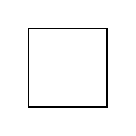
\begin{tikzpicture}[baseline]%
        \draw[black] (0,0) rectangle (\rectwidth,\rectheight);
      \end{tikzpicture}
    };
}


\begin{frame}{Distributed Function Secret Sharing: Functionality}

Distributed Function Secret Sharing functionality delivers correlated keys for two parties.

\vspace{14em}

\centering

\begin{tikzpicture}[overlay, remember picture]

% Colors
\definecolor{mygreen}{RGB}{0,150,0}
\definecolor{mypurple}{RGB}{150,60,180}

% --- Alice image ---
\node[anchor=center, xshift=-5cm, yshift=0cm]
    (aliceimg)
    at (current page.center)
    {\includegraphics[width=0.13\linewidth]{../Resources/Alice.png}};

% --- Bob image ---
\node[anchor=center, xshift=5cm, yshift=0cm]
    (bobimg)
    at (current page.center)
    {\includegraphics[width=0.15\linewidth]{../Resources/Bob.png}};

% --- Oracle image ---
\node[anchor=center, xshift=0.3cm, yshift=0cm]
    (oracleimg)
    at (current page.center)
    {\includegraphics[width=0.4\linewidth]{../Resources/Oracle.png}};

% --- Arrows + labels -----------------------------------------
\draw[->, thick, mygreen]
  ([yshift=0.5cm] aliceimg.east) to[out=30,in=150] ([xshift=2.8cm, yshift=0.5cm] aliceimg.east);
\node[text=mypurple] at ([xshift=1.3cm,yshift=0.65cm] aliceimg.east) {{\scriptsize interval}};
\node at ([xshift=1.3cm,yshift=1.03cm] aliceimg.east) {{\scriptsize $\alpha$}};

\draw[->, thick, mygreen]
  ([yshift=0.5cm] bobimg.west) to[out=150,in=30] ([xshift=-2.6cm, yshift=0.5cm] bobimg.west);
\node[text=mypurple] at ([xshift=-1.3cm,yshift=0.65cm] bobimg.west) {{\scriptsize payload}};
\node at ([xshift=-1.3cm,yshift=1.03cm] bobimg.west) {{\scriptsize $\beta \in \{0, 1\}^\kappa$}};

% Output arrows
\visible<2>{
\draw[<-, thick, mygreen]
  ([yshift=-0.5cm] aliceimg.east) to[out=-30,in=-150] ([xshift=2.8cm, yshift=-0.5cm] aliceimg.east);
\node at ([xshift=1.3cm,yshift=-1.15cm] aliceimg.east)
  {\includegraphics[width=0.07\linewidth]{../Resources/Key_mirrored.png}};
\node at ([xshift=1.55cm,yshift=-1.4cm] aliceimg.east) {{\scriptsize $0$}};

\draw[<-, thick, mygreen]
  ([yshift=-0.5cm] bobimg.west) to[out=-150,in=-30] ([xshift=-2.6cm, yshift=-0.5cm] bobimg.west);
\node at ([xshift=-1.3cm,yshift=-1.15cm] bobimg.west)
  {\includegraphics[width=0.07\linewidth]{../Resources/Key_mirrored.png}};
\node at ([xshift=-1.35cm,yshift=-1.4cm] bobimg.west) {{\scriptsize $1$}};
}
\end{tikzpicture}

\end{frame}

\begin{frame}
\frametitle{Cost has changed}
From {\color{orange} $\kappa$} FSS key generations to {\color{teal} $1$} distributed FSS.
\vspace{15em}
\begin{tikzpicture}[overlay, remember picture]
\definecolor{mygreen}{RGB}{0,150,0}
\definecolor{mypurple}{RGB}{150,60,180}

  % --- Alice image ---
\node[anchor=center, xshift=-6cm, yshift=-2cm]
    (aliceimg)
    at (current page.center)
    {\includegraphics[width=0.13\linewidth]{../Resources/Alice.png}};

% --- Bob image ---
\node[anchor=center, xshift=6cm, yshift=-2cm]
    (bobimg)
    at (current page.center)
    {\includegraphics[width=0.13\linewidth]{../Resources/Bob.png}};

%% --- Axis line ---
\draw[-, thick] ([xshift=-1cm, yshift=-0.5cm] aliceimg.south) -- ([xshift=2.5cm, yshift=-0.5cm] aliceimg.south);

%% --- Red interval (Alice interval) ---
\draw[line width=3pt, red!60, rounded corners=3pt] ([xshift=-1cm, yshift=-0.53cm] aliceimg.south) -- ([xshift=1.3cm, yshift=-0.53cm] aliceimg.south);

\only<1>{
\node (key0A) at ([xshift=2cm,yshift=2.9cm] aliceimg.east) 
  {\includegraphics[width=0.07\linewidth]{../Resources/redkey_mirror.png}};
\node at ([xshift=0.15cm,yshift=0.15cm] key0A.south) {$\textcolor{red}{0}$};

\node (key1A) at ([xshift=2.8cm,yshift=2.9cm] aliceimg.east) 
  {\includegraphics[width=0.07\linewidth]{../Resources/redkey_mirror.png}};
\node at ([xshift=0.15cm,yshift=0.15cm] key1A.south) {$\textcolor{red}{1}$};\draw[->, thick]
([yshift=2.2cm] aliceimg.east) to[out=10,in=170] ([xshift=4.3cm, yshift=2.2cm] aliceimg.east);\node (oracleA) 
  at ([yshift=2.2cm, xshift=4.9cm] aliceimg.east)
  {\includegraphics[width=0.2\linewidth]{../Resources/Oracle.png}};\draw[->, thick]
([yshift=2.2cm] bobimg.west) to[out=170,in=10] ([xshift=-4cm, yshift=2.2cm] bobimg.west);
\node at ([yshift=2.7cm,xshift=-2.1cm] bobimg.west) {$\textcolor{red}{b_1} \gets \$$};
\draw[<-, thick]
  ([yshift=2.1cm] bobimg.west) to[out=-170,in=-10] ([xshift=-4cm, yshift=2.1cm] bobimg.west);
\node (keybA) at ([yshift=1.7cm,xshift=-0.3cm] bobimg.west)
  {\includegraphics[width=0.07\linewidth]{../Resources/redkey_mirror.png}};
\node at ([xshift=0.15cm,yshift=0.15cm] keybA.south) {{\color{red} $b_1$}};

% Instance 2 (middle)
  \node (key0B) at ([xshift=2cm,yshift=1.5cm] aliceimg.east) 
    {\includegraphics[width=0.07\linewidth]{../Resources/bluekey_mirror.png}};
  \node at ([xshift=0.15cm,yshift=0.15cm] key0B.south) {$\textcolor{blue}{0}$};

  \node (key1B) at ([xshift=2.8cm,yshift=1.5cm] aliceimg.east) 
    {\includegraphics[width=0.07\linewidth]{../Resources/bluekey_mirror.png}};
  \node at ([xshift=0.15cm,yshift=0.15cm] key1B.south) {$\textcolor{blue}{1}$};
\draw[->, thick]
  ([yshift=0.8cm] aliceimg.east) to[out=10,in=170] ([xshift=4.3cm, yshift=0.8cm] aliceimg.east);
\node (oracleB) 
    at ([yshift=0.8cm, xshift=4.9cm] aliceimg.east)
    {\includegraphics[width=0.2\linewidth]{../Resources/Oracle.png}};
\draw[->, thick]
  ([yshift=0.8cm] bobimg.west) to[out=170,in=10] ([xshift=-4cm, yshift=0.8cm] bobimg.west);
\node at ([yshift=1.3cm,xshift=-2.1cm] bobimg.west) {$\textcolor{blue}{b_2} \gets \$$};
\draw[<-, thick]
  ([yshift=0.7cm] bobimg.west) to[out=-170,in=-10] ([xshift=-4cm, yshift=0.7cm] bobimg.west);
\node (keybB) at ([yshift=0.3cm,xshift=-0.3cm] bobimg.west)
  {\includegraphics[width=0.07\linewidth]{../Resources/bluekey_mirror.png}};
\node at ([xshift=0.15cm,yshift=0.15cm] keybB.south) {{\color{blue} $b_2$}};

% Dots separating second and third
  \node at ([yshift=-0.3cm, xshift=4.9cm] aliceimg.east) {$\vdots$};
  \node at ([yshift=-0.3cm, xshift=5.7cm] aliceimg.east) {{\scriptsize $\kappa$ times}};

% Instance 3 (bottom)
  \node (key0C) at ([xshift=2cm,yshift=-0.2cm] aliceimg.east) 
    {\includegraphics[width=0.07\linewidth]{../Resources/blackkey_mirror.png}};
  \node at ([xshift=0.15cm,yshift=0.15cm] key0C.south) {$0$};

  \node (key1C) at ([xshift=2.8cm,yshift=-0.2cm] aliceimg.east) 
    {\includegraphics[width=0.07\linewidth]{../Resources/blackkey_mirror.png}};
\node at ([xshift=0.15cm,yshift=0.15cm] key1C.south) {$1$};
\draw[->, thick]
  ([yshift=-0.9cm] aliceimg.east) to[out=10,in=170] ([xshift=4.3cm, yshift=-0.9cm] aliceimg.east);
\node (oracleC) 
    at ([yshift=-0.9cm, xshift=4.9cm] aliceimg.east)
    {\includegraphics[width=0.2\linewidth]{../Resources/Oracle.png}};
\draw[->, thick]
  ([yshift=-0.9cm] bobimg.west) to[out=170,in=10] ([xshift=-4cm, yshift=-0.9cm] bobimg.west);
  \node at ([yshift=-0.4cm,xshift=-2.1cm] bobimg.west) {$\textcolor{black}{b_\kappa} \gets \$$};
  \draw[<-, thick]
    ([yshift=-1.0cm] bobimg.west) to[out=-170,in=-10] ([xshift=-4cm, yshift=-1.0cm] bobimg.west);
  \node (keybC) at ([yshift=-1.4cm,xshift=-0.3cm] bobimg.west)
    {\includegraphics[width=0.07\linewidth]{../Resources/blackkey_mirror.png}};
\node at ([xshift=0.15cm,yshift=0.15cm] keybC.south) {{\color{black} $b_\kappa$}};
}

\only<2>{
% --- Oracle image ---
\node[anchor=center, xshift=0.3cm, yshift=-2cm]
    (oracleimg)
    at (current page.center)
    {\includegraphics[width=0.4\linewidth]{../Resources/Oracle.png}};

% --- Arrows + labels -----------------------------------------
\draw[->, thick, mygreen]
  ([yshift=0.5cm] aliceimg.east) to[out=30,in=150] ([xshift=2.8cm, yshift=0.5cm] aliceimg.east);
\node[text=mypurple] at ([xshift=1.3cm,yshift=0.65cm] aliceimg.east) {{\scriptsize interval}};
\node at ([xshift=1.3cm,yshift=1.03cm] aliceimg.east) {{\scriptsize $\alpha$}};

\draw[->, thick, mygreen]
  ([yshift=0.5cm] bobimg.west) to[out=150,in=30] ([xshift=-2.6cm, yshift=0.5cm] bobimg.west);
\node[text=mypurple] at ([xshift=-1.3cm,yshift=0.65cm] bobimg.west) {{\scriptsize payload}};
\node at ([xshift=-1.3cm,yshift=1.03cm] bobimg.west) {{\scriptsize $\beta \in \{0, 1\}^\kappa$}};

\node[text width=3.5cm, align=right] (entropyNote) at ([xshift=0.2cm,yshift=3.0cm] bobimg.west) {{\scriptsize Entropies of choice bits $b_1, \ldots, b_\kappa$ moved here}};
\draw[->, thick, mygreen]
  (entropyNote.south) to[out=-10,in=150] ([xshift=-1.3cm,yshift=1.23cm] bobimg.west);

% Output arrows
\draw[<-, thick, mygreen]
  ([yshift=-0.5cm] aliceimg.east) to[out=-30,in=-150] ([xshift=2.8cm, yshift=-0.5cm] aliceimg.east);
\node at ([xshift=1.3cm,yshift=-1.15cm] aliceimg.east)
  {\includegraphics[width=0.07\linewidth]{../Resources/Key_mirrored.png}};
\node at ([xshift=1.55cm,yshift=-1.4cm] aliceimg.east) {{\scriptsize $0$}};

\draw[<-, thick, mygreen]
  ([yshift=-0.5cm] bobimg.west) to[out=-150,in=-30] ([xshift=-2.6cm, yshift=-0.5cm] bobimg.west);
\node at ([xshift=-1.3cm,yshift=-1.15cm] bobimg.west)
  {\includegraphics[width=0.07\linewidth]{../Resources/Key_mirrored.png}};
\node at ([xshift=-1.35cm,yshift=-1.4cm] bobimg.west) {{\scriptsize $1$}};
}

\end{tikzpicture}

\end{frame}

\begin{frame}
\frametitle{Distributed Function Secret Sharing: Construction}
\only<1>{
Construction similar to prior works on Distributed Point Function \cite{doerner2017scaling}. \\
Bob has a tree, each node contains one {\color{brown} seed} and one {\color{orange} payload}.
}
\only<2>{
From the root {\color{brown} seed}, Bob gradually expands later {\color{brown} seeds} and {\color{orange} payloads} with PRG (\`a la GGM tree).
Evaluation result of $x$ is {\color{orange} aggregation of payloads} from root to the corresponding leaf.
}
\only<3>{
For points $x \le \alpha$, Alice wants to learn the exact {\color{orange} aggregation}. \\
For points $x > \alpha$, Alice wants to learn {\color{orange} aggregation $\oplus \beta$}.
}
\only<4>{
Just need {\color{teal} critical path} and its neighbors. \\
Alice learns these with Oblivious Transfer.
}
\vspace{17em}
\begin{tikzpicture}[overlay, remember picture]
  % --- Alice image ---
  \node[anchor=north west, xshift=3.0cm, yshift=-2.5cm]
      (aliceimg)
      at (current page.north west)
      {\includegraphics[width=0.10\linewidth]{../Resources/Alice.png}};

  % --- Bob image ---
  \node[anchor=north east, xshift=-3.0cm, yshift=-2.5cm]
      (bobimg)
      at (current page.north east)
      {\includegraphics[width=0.11\linewidth]{../Resources/Bob.png}};

  % --- Bob's tree (8 leaves) ---
  % root
  \rectnode{node00l}{brown}{-\rectwidth}{-0.8}{bobimg};
  \rectnode{node00r}{orange}{\rectwidth}{0.1}{node00l};

  % 1st layer
  \rectnode{node10l}{brown}{-1.5-\rectwidth}{-1.8}{bobimg};
  \rectnode{node10r}{orange}{\rectwidth}{0.1}{node10l};

  \rectnode{node11l}{brown}{1.5-\rectwidth}{-1.8}{bobimg};
  \rectnode{node11r}{orange}{\rectwidth}{0.1}{node11l};

  % 2nd layer
  \rectnode{node20l}{brown}{-2.2-\rectwidth}{-2.8}{bobimg};
  \rectnode{node20r}{orange}{\rectwidth}{0.1}{node20l};

  \rectnode{node21l}{brown}{-0.8-\rectwidth}{-2.8}{bobimg};
  \rectnode{node21r}{orange}{\rectwidth}{0.1}{node21l};

  \rectnode{node22l}{brown}{0.8-\rectwidth}{-2.8}{bobimg};
  \rectnode{node22r}{orange}{\rectwidth}{0.1}{node22l};

  \rectnode{node23l}{brown}{2.2-\rectwidth}{-2.8}{bobimg};
  \rectnode{node23r}{orange}{\rectwidth}{0.1}{node23l};

  % 3rd layer
  \rectnode{node30l}{brown}{-2.55-\rectwidth}{-3.8}{bobimg};
  \rectnode{node30r}{orange}{\rectwidth}{0.1}{node30l};

  \rectnode{node31l}{brown}{-1.85-\rectwidth}{-3.8}{bobimg};
  \rectnode{node31r}{orange}{\rectwidth}{0.1}{node31l};

  \rectnode{node32l}{brown}{-1.15-\rectwidth}{-3.8}{bobimg};
  \rectnode{node32r}{orange}{\rectwidth}{0.1}{node32l};

  \rectnode{node33l}{brown}{-0.45-\rectwidth}{-3.8}{bobimg};
  \rectnode{node33r}{orange}{\rectwidth}{0.1}{node33l};

  \rectnode{node34l}{brown}{0.45-\rectwidth}{-3.8}{bobimg};
  \rectnode{node34r}{orange}{\rectwidth}{0.1}{node34l};

  \rectnode{node35l}{brown}{1.15-\rectwidth}{-3.8}{bobimg};
  \rectnode{node35r}{orange}{\rectwidth}{0.1}{node35l};

  \rectnode{node36l}{brown}{1.85-\rectwidth}{-3.8}{bobimg};
  \rectnode{node36r}{orange}{\rectwidth}{0.1}{node36l};

  \rectnode{node37l}{brown}{2.55-\rectwidth}{-3.8}{bobimg};
  \rectnode{node37r}{orange}{\rectwidth}{0.1}{node37l};

  \visible<2,3>{
    % Curved path to the first leaf, combining payloads (orange nodes)
    \draw[->, very thick, orange!80!black]
      (node00r.south) to[out=-140,in=40] node[midway, fill=white, inner sep=1pt] {$\oplus$} (node10r.north);
    \draw[->, very thick, orange!80!black]
      (node10r.south) to[out=-150,in=30] node[midway, fill=white, inner sep=1pt] {$\oplus$} (node20r.north);
    \draw[->, very thick, orange!80!black]
      (node20r.south) to[out=-140,in=40] node[midway, fill=white, inner sep=1pt] {$\oplus$} (node30r.north);
  }

  \only<1,2,3>{
    % Alice's hollow tree (8 leaves)
    % root
    \rectnodehollow{anode00l}{\rectwidth}{-0.8}{aliceimg};
    \rectnodehollow{anode00r}{\rectwidth}{0.1}{anode00l};

    % 1st layer
    \rectnodehollow{anode10l}{1.5+\rectwidth}{-1.8}{aliceimg};
    \rectnodehollow{anode10r}{\rectwidth}{0.1}{anode10l};

    \rectnodehollow{anode11l}{-1.5+\rectwidth}{-1.8}{aliceimg};
    \rectnodehollow{anode11r}{\rectwidth}{0.1}{anode11l};

    % 2nd layer
    \rectnodehollow{anode20l}{2.2+\rectwidth}{-2.8}{aliceimg};
    \rectnodehollow{anode20r}{\rectwidth}{0.1}{anode20l};

    \rectnodehollow{anode21l}{0.8+\rectwidth}{-2.8}{aliceimg};
    \rectnodehollow{anode21r}{\rectwidth}{0.1}{anode21l};

    \rectnodehollow{anode22l}{-0.8+\rectwidth}{-2.8}{aliceimg};
    \rectnodehollow{anode22r}{\rectwidth}{0.1}{anode22l};

    \rectnodehollow{anode23l}{-2.2+\rectwidth}{-2.8}{aliceimg};
    \rectnodehollow{anode23r}{\rectwidth}{0.1}{anode23l};

    % 3rd layer
    \rectnodehollow{anode30l}{2.55+\rectwidth}{-3.8}{aliceimg};
    \rectnodehollow{anode30r}{\rectwidth}{0.1}{anode30l};

    \rectnodehollow{anode31l}{1.85+\rectwidth}{-3.8}{aliceimg};
    \rectnodehollow{anode31r}{\rectwidth}{0.1}{anode31l};

    \rectnodehollow{anode32l}{1.15+\rectwidth}{-3.8}{aliceimg};
    \rectnodehollow{anode32r}{\rectwidth}{0.1}{anode32l};

    \rectnodehollow{anode33l}{0.45+\rectwidth}{-3.8}{aliceimg};
    \rectnodehollow{anode33r}{\rectwidth}{0.1}{anode33l};

    \rectnodehollow{anode34l}{-0.45+\rectwidth}{-3.8}{aliceimg};
    \rectnodehollow{anode34r}{\rectwidth}{0.1}{anode34l};

    \rectnodehollow{anode35l}{-1.15+\rectwidth}{-3.8}{aliceimg};
    \rectnodehollow{anode35r}{\rectwidth}{0.1}{anode35l};

    \rectnodehollow{anode36l}{-1.85+\rectwidth}{-3.8}{aliceimg};
    \rectnodehollow{anode36r}{\rectwidth}{0.1}{anode36l};

    \rectnodehollow{anode37l}{-2.55+\rectwidth}{-3.8}{aliceimg};
    \rectnodehollow{anode37r}{\rectwidth}{0.1}{anode37l};
  }

\only<4>{
  % Alice's tree with highlighted critical path to the 6th leaf (node32) and neighbors
  % root
  \rectnode{anode00l}{brown}{\rectwidth}{-0.8}{aliceimg};
  \rectnode{anode00r}{orange}{\rectwidth}{0.1}{anode00l};

  % 1st layer (path node + neighbor)
  \rectnode{anode10l}{brown}{1.5+\rectwidth}{-1.8}{aliceimg}; % on path
  \rectnode{anode10r}{orange}{\rectwidth}{0.1}{anode10l};

  \rectnode{anode11l}{brown!30}{-1.5+\rectwidth}{-1.8}{aliceimg}; % neighbor
  \rectnode{anode11r}{orange!30}{\rectwidth}{0.1}{anode11l};

  % 2nd layer (path node + neighbors)
  \rectnode{anode20l}{brown!30}{2.2+\rectwidth}{-2.8}{aliceimg}; % sibling of path
  \rectnode{anode20r}{orange!30}{\rectwidth}{0.1}{anode20l};

  \rectnode{anode21l}{brown}{0.8+\rectwidth}{-2.8}{aliceimg}; % on path
  \rectnode{anode21r}{orange}{\rectwidth}{0.1}{anode21l};

  \rectnode{anode22l}{brown!30}{-0.8+\rectwidth}{-2.8}{aliceimg}; % neighbor
  \rectnode{anode22r}{orange!30}{\rectwidth}{0.1}{anode22l};

  \rectnodehollow{anode23l}{-2.2+\rectwidth}{-2.8}{aliceimg};
  \rectnodehollow{anode23r}{\rectwidth}{0.1}{anode23l};

  % 3rd layer (path leaf = 6th leaf, its sibling, others hollow)
  \rectnodehollow{anode30l}{2.55+\rectwidth}{-3.8}{aliceimg};
  \rectnodehollow{anode30r}{\rectwidth}{0.1}{anode30l};

  \rectnodehollow{anode31l}{1.85+\rectwidth}{-3.8}{aliceimg};
  \rectnodehollow{anode31r}{\rectwidth}{0.1}{anode31l};

  \rectnode{anode32l}{brown}{1.15+\rectwidth}{-3.8}{aliceimg}; % 6th leaf seed
  \rectnode{anode32r}{orange}{\rectwidth}{0.1}{anode32l};      % 6th leaf payload

  \rectnode{anode33l}{brown!30}{0.45+\rectwidth}{-3.8}{aliceimg}; % sibling leaf
  \rectnode{anode33r}{orange!30}{\rectwidth}{0.1}{anode33l};

  \rectnodehollow{anode34l}{-0.45+\rectwidth}{-3.8}{aliceimg};
  \rectnodehollow{anode34r}{\rectwidth}{0.1}{anode34l};

  \rectnodehollow{anode35l}{-1.15+\rectwidth}{-3.8}{aliceimg};
  \rectnodehollow{anode35r}{\rectwidth}{0.1}{anode35l};

  \rectnodehollow{anode36l}{-1.85+\rectwidth}{-3.8}{aliceimg};
  \rectnodehollow{anode36r}{\rectwidth}{0.1}{anode36l};

  \rectnodehollow{anode37l}{-2.55+\rectwidth}{-3.8}{aliceimg};
  \rectnodehollow{anode37r}{\rectwidth}{0.1}{anode37l};
}

\end{tikzpicture}

\end{frame}

\begin{frame}
\frametitle{Related Works}
\textbf{Fuzzy Private Set Intersection}: Techniques based on:
\begin{itemize}
    \item GC or FHE: \cite{richardson2024fuzzy, son2025doubly, uzun2021fuzzy}.
    \item AHE: \cite{van2024fuzzy, gao2024efficient}.
    \item Symmetric Key: \cite{zhang2025fast}, \\
          \quad \quad \cite{van2025fuzzy}.
\end{itemize}
\textbf{Structure-Aware Private Set Intersection:}
\begin{itemize}
  \item FSS: \cite{garimella2022structure,garimella2024computation}.
  \item FSS, Malicious: \cite{garimella2023malicious}.
  \item Still FSS: This work.
\end{itemize}

\end{frame}

\begin{frame}[plain]
\setbeamercolor{background canvas}{bg=white}

\begin{tikzpicture}[remember picture,overlay]

% ---- MAIN TITLE ----
\node[anchor=center] at ([yshift=20mm]current page.center) {
    \begin{minipage}{\linewidth}
        \centering
        {\LARGE\bfseries New Framework for Structure-Aware PSI \\[2mm]
        from Distributed Function Secret Sharing}
    \end{minipage}
};

% ---- AUTHORS (no institutions) ----
\node[anchor=center] at ([yshift=3mm]current page.center) {
    \begin{minipage}{0.9\linewidth}
        \centering
        {\large
            Dung Bui \quad
            Gayathri Garimella \quad
            Peihan Miao \quad
            Phuoc Pham
        }
    \end{minipage}
};

% ---- CONFERENCE NAME (moved up) ----
\node[anchor=center] at ([yshift=-12mm]current page.center) {
    {\large Asiacrypt 2025}
};

% ---- Links ----
\node[anchor=center] (paperlink) at ([yshift=-22mm]current page.center) {\small Paper: \texttt{https://eprint.iacr.org/2025/907}};
\node[anchor=center] (githublink) at ([yshift=-30mm]current page.center) {\small Implementation: \texttt{https://github.com/phuocchubeo123/SaPSI.git}};

% ---- Artifact callout ----
\node[anchor=west, text=darkgreen] (artifact) at ([xshift=3.2cm,yshift=-1cm]current page.center) {\small Asiacrypt 2025 Artifact!};
\draw[->, thick, darkgreen] (githublink.east) to[out=10,in=170] (artifact.west);

\end{tikzpicture}
\end{frame}

\begin{frame}[allowframebreaks]
\footnotesize
    \bibliography{refs}
\end{frame}

\end{document}
